\chapter{One-Group Reactor Methodology}
\index{One-Group Reactor Methodology@\emph{One-Group Reactor Methodology}}
\label{1g_paper}



\section{Introduction}
\index{Introduction@\emph{Introduction}}
\label{1g_sec:intro}
High fidelity coupled neutron transport and fuel burnup calculations require large execution times
and intensive computational resources.  This constraint renders such calculations impractical when 
it is desired to address high level fuel cycle engineering problems on a reasonable time scale.  
The approaches taken in the past to circumvent these time constraints have typically sacrificed 
fidelity by fully decoupling the fuel cycle simulation from physics-based reactor burnup calculations [1].  

Fuel cycle problems revolve around finding the optimum value for a parameter in order to achieve a certain 
global result.  For instance, initial fresh fuel compositions in a reactor may be varied to attain a specific 
burnup. Or repository impact may be of more concern so cooling time before emplacement may be varied.  Even 
the simplest once-through fuel cycle on an isotopic level has a large number of degrees of freedom, each 
featuring a continuum of acceptable values.  Lengthy calculation times for input and output fuel vectors 
in the fuel cycles reactor or reactors make a real parameterization of these degrees of freedom a near 
impossibility.  

Rather than relying on predetermined recipes that limit study to specific cores with precise burnups, 
there is a need for a medium fidelity mechanism that allows for quick, dynamic calculation of burnup 
parameters.  The methodology that is described within details a tool for use in fuel cycle analyses 
that calculates these burnup-related parameters for any arbitrary reactor or interacting fleet of reactors.

The burnup-related parameters include at least the input and output isotopic vectors for the reactor 
as well as the burnup itself, which in turn depends on criticality, allowable fluence, safety issues 
such as reactivity coefficient values, and other constraints.  Other parameters may be of interest 
for specific fuel cycles and will be discussed as they arise.  The burnup tool uses pre-tabulated 
values for the neutron production and destruction rates and the burnup as a function of initial 
isotope present and fluence.  The algorithm then eliminates fluence, giving the burnup only in 
terms of the initial isotopics of the reactor.  The initial isotopics of the core may be iterated 
using this process until the composition that reaches some target burnup is found.  This process 
assumes that there are multiple actinide streams to be blended, and the blending ratios are unknowns 
to be computed.  The output isotopics of the reactor are dependent on initial core composition and 
the burnup, and thus are calculated after other parameters.   This tool may then be embedded within 
a full fuel cycle model.  To demonstrate how such a coupled framework functions, it is applied to 
two fuel cycle concepts.  

The first of the two fuel cycles incorporates a limited uranium recycle strategy.   Uranium from a 
standard pressurized water reactor (PWR) is reprocessed and blended with enriched natural uranium 
(NU) before going into the second core to be burned again.  After this burn, it is noteworthy that 
further recycling via blending is still possible.  In other words, this fuel cycle could be fully 
closed with respect to the uranium stream, avoiding the need to dispose of the reprocessed uranium 
that comprises over 90\% of the mass of spent PWR fuel on an initial heavy metal (IHM) basis.  
This is known as a recyclable uranium (RU) blend and burn fuel cycle since the uranium is reused 
in PWRs, independently of other actinides.  RU blend and burn is an attractive option since it has 
the potential to eventually do a near complete burn of all uranium in LWR spent fuel if used in a 
fully closed cycle.

The second fuel cycle that utilizes the burnup tool developed here demonstrates how the tool may 
be used to improve the fidelity of the fuel cycle material balance calculations associated with 
one of the Global Nuclear Energy Partnership (GNEP) base-case proposals [2].  This case is a 
closed fuel cycle that uses a fast burner reactor (FR) with a conversion ratio of 0.5.  
Actinides are continually recycled in the FR while fission products (FP) are removed and 
disposed.  The reprocessing facility that is built for fast reactor spent fuel has a separation 
efficiency of 0.99 for all actinides.  This is a meaningful option to explore since fast reactors 
are considered to be a key component of long term nuclear energy strategies that close the fuel cycle.

In these two instances the same basic algorithm is used to very quickly solve the blending problem 
to obtain the fresh fuel composition that achieves the desired discharge burnup (BUd); the isotopic 
content of the output is also calculated.   A fuel cycle wrapper governs the mass streams through 
the reactors and other fuel cycle components.  

As will be seen, many fuel cycle parameters may be calculated from the resulting data.  Moreover 
due to the dynamic nature of this method, these parameters will be more accurate and meaningful 
than if a static recipe or simple linearization had been used.  A static recipe would not be able 
to mix recyclable and low enriched uranium (LEU) streams in a way that respects the dependence of 
neutronic characteristics on feed composition, an issue that is inherent to the RU fuel cycle.  
Moreover, models that use static recipes may fail to accurately capture the evolution of material 
balances with each successive pass through a fast reactor.   

The remainder of this paper proceeds via the following layout. The next and second section is a 
full illustration of the burnup model.  The third section is discusses the in depth the recyclable 
uranium and fast reactor fuel cycles to which the burnup model is applied.  The fourth section 
presents the results obtained for these cycles.  The fifth and final section is concludes this 
study and discusses opportunities for future work. 




\section{Burnup Model}
\index{Burnup Model@\emph{Burnup Model}}
\label{1g_sec:bu_model}
The burnup model takes a given input isotopic composition and returns the maximum discharge 
burnup of the fuel as well as its post-irradiation isotopic composition.  Thus, if given a 
target burnup, the model can mix multiple material streams to solve for the fresh fuel composition 
that achieves this burnup.

To form the basis for the burnup model algorithm, certain quantities are assumed to be known.  
The neutron production and destruction rates, the burnup, and the compositional evolution of 
every isotope initially present, namely the actinides and the coolant, are given.  Furthermore, 
they are all specified as functions of fluence (F), the time integral of the total spatially-averaged 
flux in the reactor. A discussion of how to compute and compile these presupposed parameters follows 
later in the burnup model section. 


\subsection{Isotopic Transformation}
\index{Isotopic Transformation@\emph{Isotopic Transformation}}
\label{1g_sec:iso_transform}
The first of the known burnup model parameters is nuclide-specific isotopic transformation as a 
function of fluence, $T_{ij}(F)$ [kg\subscript{j}/kg\subscript{i}].  The subscript $i$ denotes 
the isotope initially present in the core, where as the subscript $j$ labels those nuclides bred in.  
The $T_{ij}(F)$ hence track the transmutation under fluence of the ith isotope into its daughters 
given a nominal reactor spectrum embodied by one-group cross sections.  The daughters tracked 
include both fission products (FP) as well and transuranics (TRU).
\begin{figure}[htbp]
\caption{\nuc{Pu}{239} Transformation as a Function of Fluence for a Sample Fast Reactor}
\label{1g_fig01}
\begin{center}
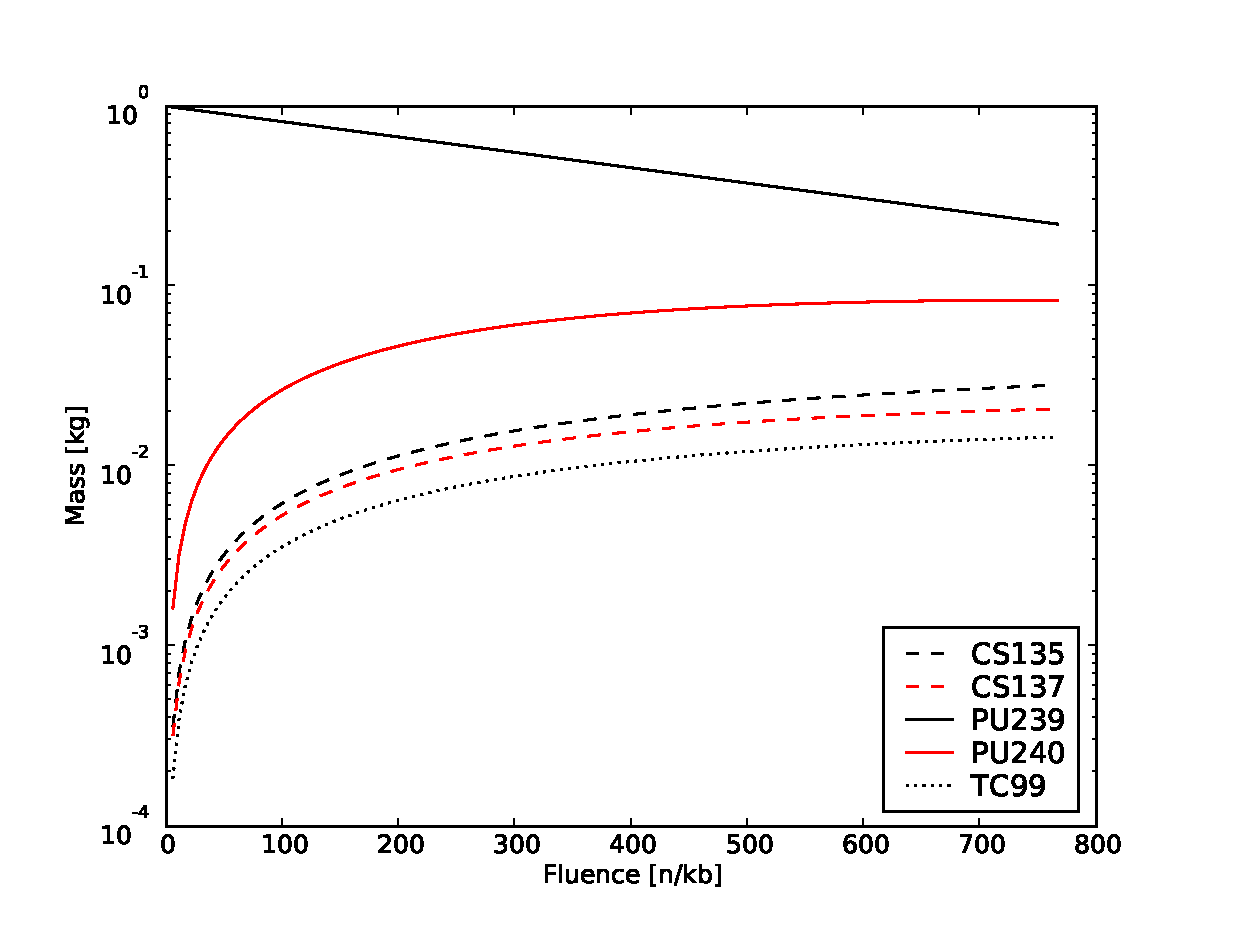
\includegraphics[scale=0.5]{one_group_method/figs/Fig01.eps}
\end{center}
\end{figure}
Figure \ref{1g_fig01} displays an example of this transformation data: the concentration in 
kilograms of tracked isotopes that are present in a sodium-cooled FR core as a function of 1 kg 
of the initial isotope (\nuc{Pu}{239} in this illustration).  In the figure, only one isotope 
(\nuc{Pu}{239} here) is non-zero at zero fluence (ie zero time in the reactor).  For each 
distinct reactor and general fuel type, similar data are required for all other transmuting 
nuclides initially present.   Note that not all species that \nuc{Pu}{239} transforms into are displayed. 

Since this example is for fast reactors, a constant flux of $2\times10^{15}$ [n/cm2/s] was used 
when generating the transformation matrices.  For PWRs a constant flux of was $4\times10^{14}$ [n/cm2/s] 
assumed.  The units of fluence ($F$) here are [neutrons/kilobarn], abbreviated [n/kb], while the 
flux ($\phi$) is again [n/cm2/s], and time ($t$) is given in [days].
\begin{equation}
\label{fluence}
F = \int_0^t \phi dt^\prime = \phi \int_0^t dt^\prime = \phi \times t \cdot \frac{24 \cdot 3600 \cdot 10^3}{10^{24}}
\end{equation}
In practice, the $T_{ij}$ data need only exist for the actinides because coolant and structural 
material transmutation does not significantly impact core neutronic performance.

From here it is simple to apply initial isotopic weight fractions and superposition to Figure \ref{1g_fig01}
and its analogies for all isotopes initially present in the core.  This superimposed result then describes 
how 1 kg of fresh fuel transforms as a function of fluence within the core. Once the burnup model is applied, 
the output fluence will also be known, as described below.  Plugging this fluence into the combined data 
yields the isotopic composition of the fuel at removal. 



\subsection{Neutron Production \& Destruction Rates and Burnup}
\index{Neutron Production \& Destruction Rates and Burnup@\emph{Neutron Production \& Destruction Rates and Burnup}}
\label{1g_sec:pdbu}
Other assumed fuel cycle parameters that are required to perform burnup calculations are the neutron 
production and destruction rates, $p_i(F)$ and $d_i(F)$ [n/s/flux/kg\superscript{i}].  These are given 
as functions of fluence for each isotope initially present in the core, just as with the isotopic 
transformation data.  An example of these parameters is shown in Figure \ref{1g_fig02}.
\begin{figure}[htbp]
\caption{Sample Neutron Production and Destruction Rate Figure as a Function of Fluence for an Initial Unit Mass of \nuc{Pu}{239} in a Sample Fast Reactor}
\label{1g_fig02}
\begin{center}
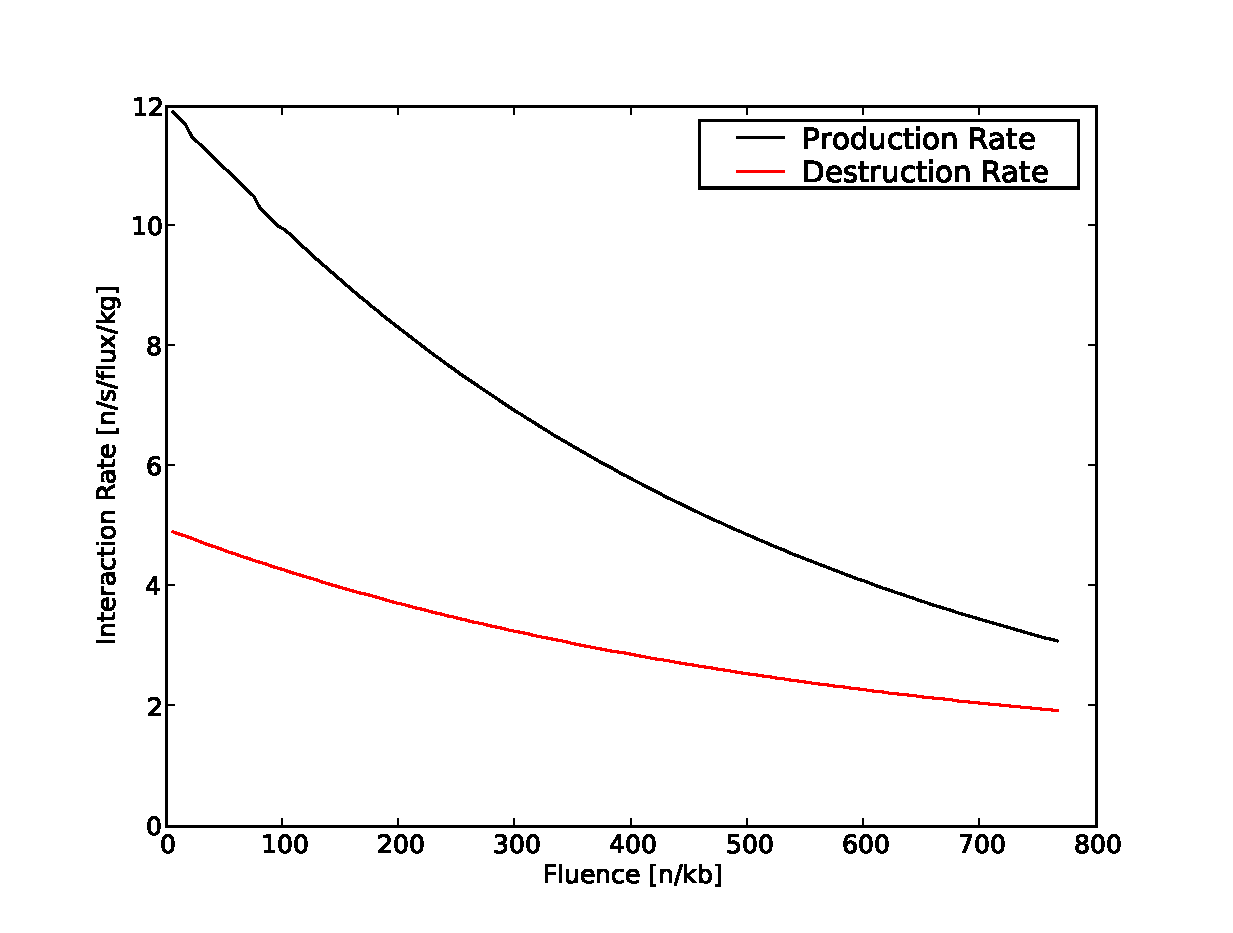
\includegraphics[scale=0.5]{one_group_method/figs/Fig02.eps}
\end{center}
\end{figure}
This figure displays the production and destruction rates for one initial kilogram of \nuc{Pu}{239} 
in the sodium-cooled FR.  Lastly, the specific burnup for each isotope initially present, $\mbox{BU}_i(F)$ 
[MWd/kgi], is assumed known by the burnup model.  The burnup is defined in the same way as the neutron 
production and destruction rates.  It is given as a function of fluence for each nuclide initially 
present in the core.  Figure \ref{1g_fig03} displays $\mbox{BU}_i(F)$ for a few actinides that may 
be present in the fresh fuel.
\begin{figure}[htbp]
\caption{Burnup as a Function of Fluence for an Initial Unit Mass of Specific Nuclides in a Sample Fast Reactor}
\label{1g_fig03}
\begin{center}
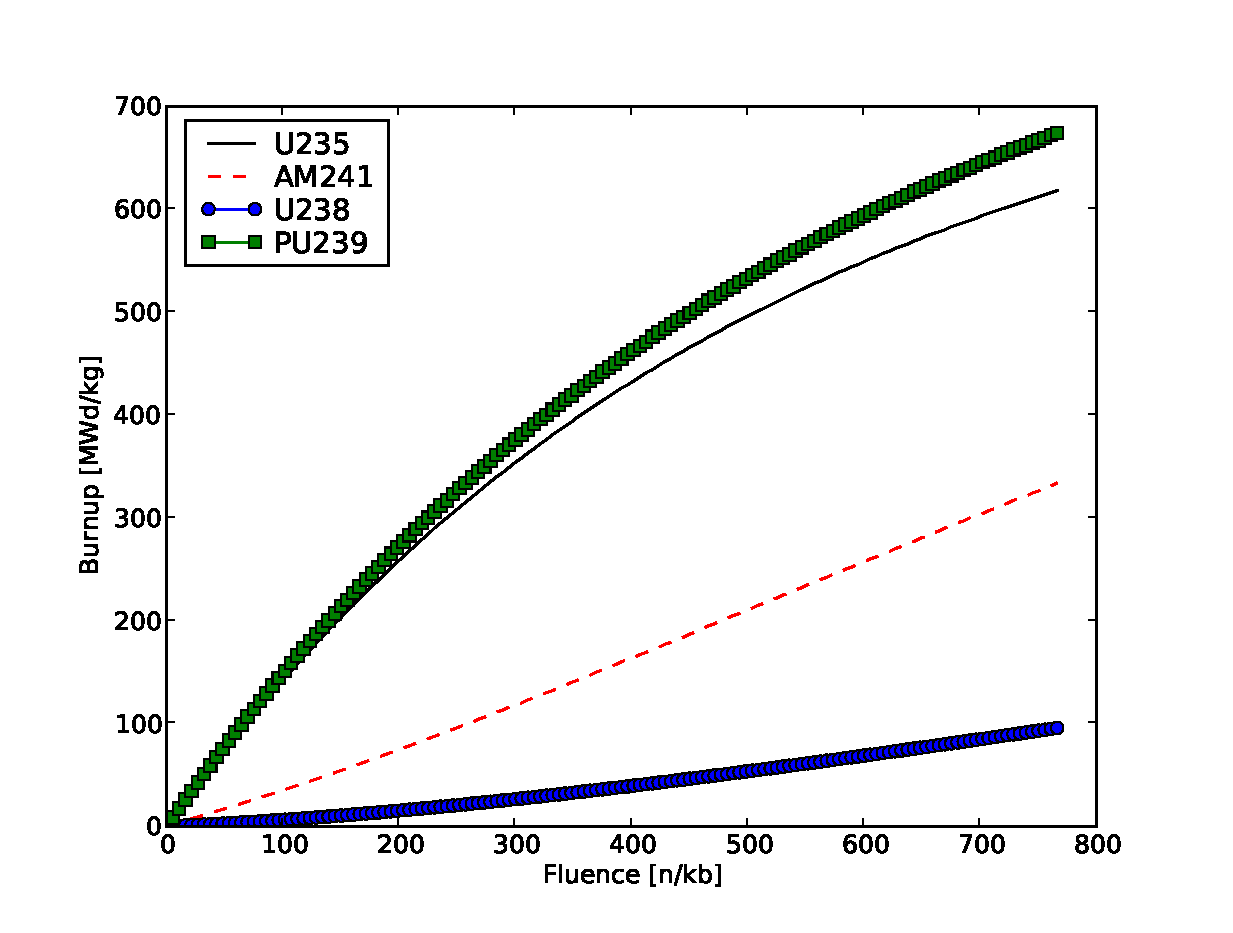
\includegraphics[scale=0.5]{one_group_method/figs/Fig03.eps}
\end{center}
\end{figure}
Now that all quantities assumed to be known have been outlined and defined, a description of the 
algorithm that calculates the discharge burnup and the input and output fuel isotopics follows.   




\subsection{Solving for BUd and Isotopics}
\index{Solving for BUd and Isotopics@\emph{Solving for BUd and Isotopics}}
\label{1g_sec:solve_BUd_iso}
First, knowing only the $\mbox{BU}_i(F)$, $p_i(F)$, $d_i(F)$, and $T_i(F)$ from the prior section, 
the maximum achievable discharge burnup, BUd [MWd/kgIHM], must be found.  The burnup of the fresh 
fuel as a function of fluence is then computed as a mass-weighted linear combination of the burnups 
from the initial constituent isotopes.  Similarly, the neutron production and destruction rates as a 
function of fluence for an arbitrary fresh fuel may also be found.  In the development below, it is 
assumed that the core consists of a lattice in which each cell contains two spatial regions, fuel ``F'' 
and coolant ``C'' but the formulation can generalize to additional regions.  Denote the mass of the 
$i$\superscript{th} isotope initially present in the fuel region ``F'' per unit mass of initial heavy 
metal (IHM) in the cell by $m_i^F$ [kg\subscript{i}/kgIHM] and the mass of the $i$\superscript{th} 
isotope initially present in the coolant region ``C'' per unit mass of initial heavy metal (IHM) by 
$m_i^C$ [kg\subscript{i}/kgIHM].  Thus for the ``Q''\superscript{th} region, the mass weights are given 
by equation \ref{Q_mass_weights}.
\begin{equation}
\label{Q_mass_weights}
m_i^Q = \frac{N_i}{N_{\mbox{IHM}}} = \frac{n_i A_i}{A_{\mbox{IHM}}} \cdot \frac{\rho^Q\cdot\mbox{MW}^F}{\rho^F\cdot\mbox{MW}^Q} \frac{V^Q}{V^F}
\end{equation}
The volumes of the fuel and coolant regions, $V^F$ and $V^C$ [cm\superscript{3}], are needed to 
compute these IHM-normalized masses and the infinite lattice of unit cell model mentioned 
above is used in modified form for this purpose.  This two region method ignores the small 
effect of the cladding material on neutron capture.  Call $r$ [cm] the radius of the fuel pin and $\ell$ [cm] 
the pitch of the unit fuel cell.  It is important to correct for the fact that not all fuel 
pin slots in a fuel assembly are filled with fuel.  Denote $S_T$ as the total number of pin 
slots in a fuel assembly and $S_O$ as the open, non-fuel containing slots.  The effective volumes 
are then given in equations \ref{1g_VF} \& \ref{1g_VC}.
\begin{equation}
\label{1g_VF}
V^F = \frac{\pi r^2}{\ell^2} \cdot \left(1 - \frac{S_O}{S_T}\right)
\end{equation}
\begin{equation}
\label{1g_VC}
V^C = \frac{\ell^2 - \pi r^2}{\ell^2} \cdot \left(1 - \frac{S_O}{S_T}\right) + \frac{S_O}{S_T}
\end{equation}
Hence the burnup of the core as a function of fluence, $\mbox{BU}(F)$ [MWd/kgIHM], is given by 
the following sum.
\begin{equation}
\label{1g_BU_F}
\mbox{BU}(F) = \sum_i m_i^F \cdot \mbox{BU}_i(F)
\end{equation}
Once this burnup is known, the maximum discharge burnup can be computed as that value of burnup 
for which the core ceases to be critical.  The fluence-dependent neutron production and destruction 
rates for each constituent are used here to compute the multiplication factor, $k$.    When $k$ drops 
below unity, a reactor full of this fuel will no longer be able to sustain a chain reaction.  $k(F)$ is 
approximated by calculating the full-core neutron production rate, $P(F)$ [n/s/kgIHM], divided by the 
full-core average neutron destruction rate, $D(F)$ [n/s/kgIHM].  Namely,
\begin{equation}
\label{1g_k_F}
k(F) = \frac{P(F)}{D(F)}
\end{equation}
$k(F)$ may thus also be calculated, like $\mbox{BU}(F)$, as a mass-weighted convolution of the $p_i(F)$ and 
$d_i(F)$.  The method by which one obtains $P(F)$ and $D(F)$ from the isotope-specific rates is discussed 
in the following sections.  However once known, $k(F)$ is then set equal to one and then equation \ref{1g_k_F} 
solved for the fluence.  This is the fluence at discharge and is called $F\mbox{d}$ [n/kb].  $F\mbox{d}$ may then 
be reinserted into equation \ref{1g_BU_F} and the burnup of the fuel composition at discharge, 
BUd [MWd/kgIHM], is attained.

Note that equation \ref{1g_k_F} can hold for a multi-batch fuel management scheme as well as a one batch core 
system.  Extending this equation to a multi-batch system follows after a discussion of the calculation of 
$P(F)$ and $D(F)$.

Additional factors complicate the calculation of the core-average neutron production and destruction rates.  
A complete depiction of the neutron balance requires that $p_i(F)$ and $d_i(F)$ for non-fuel components of 
the core must also be known.  These non-fuel components include the coolant outside of fuel regions and the 
non-actinide species in the fuel region (\emph{e.g.} oxygen in UOX).  Both of these classes of parasitic 
species serve to increase the full core destruction rate.  Disadvantage factors also affect the flux 
suppression in fuel regions which needs to be accounted for as well for PWR cases.  Furthermore, to 
account for spatial variation in the neutron flux when computing neutron interaction rates in non-fuel 
components, a general fuel assembly model is needed (as described above).  For example, to reflect a 
standard PWR fuel assembly geometry values from the OECD Burnup Credit Criticality Benchmark [3] 
were used for LWRs and nominal values for fast reactors were taken from [4].  

A walkthrough of how to calculate the core-average production and destruction rates, $P(F)$ and $D(F)$, 
from the known set of $p_i(F)$ and $d_i(F)$ for a given collection of $m_i$ now follows.  




\subsubsection{The Neutron Production Rate}
\index{The Neutron Production Rate@\emph{The Neutron Production Rate}}
\label{1g_sec:p_rate}
The $p_i(F)$ and $d_i(F)$ are superimposed to build the full-core loading.  These rates reflect the 
evolution of the neutron balance for an initial unit mass of the species $i$ when exposed to the 
neutron flux spectrum extant in the reactor being studied.  Therefore they are computed using cross 
sections prepared for a specific reactor and fresh fuel composition.

However as mentioned above, flux spectra and magnitudes are spatially dependent.  The most basic geometric 
model and the one again used is that of an infinite lattice of unit cells consisting of a central fuel region 
surrounded by a coolant-filled region.  These two regions have neutron production and destruction rates that 
are distinct since the set of mi that are used in each region is different.  Once again, use the 
superscript ``F'' to denote a parameter relating to the fuel region and the superscript ``C'' for the coolant 
region. 

The production rates for the fuel and coolant regions, $p^F(F)$ and $p^C(F)$ [n/s/flux/kgIHM], 
can be calculated in direct analogy to equation \ref{1g_BU_F} for the burnup.  The neutron production 
rate in the fuel region is 
\begin{equation}
\label{1g_pF_F}
p^F(F) = \sum_i m_i^F \cdot p_i(F)
\end{equation}
and $p^C(F) = 0$ since the coolant contains no neutron producing isotopes.  

The advantage of this algorithm is seen through equation \ref{1g_pF_F}.  By assuming that isotopic 
production and destruction rates are known, superposition is then used combine the individual rates 
into full-core or region specific rates.  This allows for fast recombining of core constituents without 
having to recalculate the isotopic rates from scratch.  For instance, to calculate the burnups achievable 
from 2\% and 4\% \nuc{U}{235} enriched PWR fuel would typically require distinct computationally intensive 
runs because of differing initial fuel compositions.  With this method all that is needed is to change the 
$m_i$ used in equation \ref{1g_pF_F} and also perhaps to obtain case-specific burnup parameters $p_i(F)$, 
$d_i(F)$ and $\mbox{BU}_i(F)$ by interpolating between a handful of precomputed sets.  

However, the fuel region production rate is not equivalent to the full-core production rate.  There is one 
core effect that is not seen at the fuel cell level: leakage.  To capture this macroscopic effect a 
non-leakage probability PNL is introduced.  The $P_{NL}$ effectively reduces the production rate of 
neutrons for the core. The PNL used is characteristic of the reactor design and composition; it may 
be computed using macroscopic transport methods, but in practice it is used as a calibration parameter.  
Finally then, the full-core production rate is given simply as 
\begin{equation}
\label{1g_P_F}
P(F) = P_{NL} \cdot p^F(F)
\end{equation}
Note that $P(F)$ here is normalized to a unit mass of IHM.  Thus $P(F)$ has units of [n/s/kgIHM], 
and the neutron destruction rate will be normalized in the same way.



\subsubsection{The Destruction Rate}
\index{The Destruction Rate@\emph{The Destruction Rate}}
\label{1g_sec:d_rate}
The full-core destruction rate, $D(F)$, is calculated in the same manner as the fuel 
region production rate.  However, the other nuclides in the reactor, while not contributing 
to fission, do contribute to neutron destruction in the core. Similarly, the burnup $\mbox{BU}_i(F)$ 
for these nuclides will also be zero since fission does not occur. In fuel cell model used above, 
two other isotopes are present in a PWR core (\nuc{O}{16} and \nuc{H}{1}) and one other main species 
in a FR core (\nuc{Na}{23}).

The following example walks through the calculation of $D(F)$.  First, start with the fuel region 
destruction rate $d^F(F)$ in analogy to the fuel region production rate equation \ref{1g_pF_F}.  Note that the 
units of $d^F(F)$ are [n/s/flux/kgIHM].  
\begin{equation}
\label{1g_dF_F}
d^F(F) = \sum_i m_i^F \cdot d_i(F)
\end{equation}
Moreover, the coolant can strongly contribute to the destruction rate.  However, it is 
important to take into account that for some fuel/coolant combinations the flux is not 
spatially uniform; for instance in PWRs the thermal flux is generally higher in the coolant 
than in the fuel. To account for this, a disadvantage factor is introduced.  For other reactor 
types, for example FRs, the flux profile is much flatter over the unit cell and a disadvantage 
factor is not necessary. The disadvantage factor $\zeta$ is qualitatively the average flux in 
the moderator divided by the average flux in the fuel. The fuel suppresses the thermal flux 
levels so $\zeta$ will always be greater than one and the flux in the moderator will always 
be greater than the flux in the fuel. Since it is dependent on the composition of the fuel, $\zeta$ 
is therefore also a function of the fluence because the fuel isotopic makeup is altered as a function 
of fluence. A fuller look at how to calculate $\zeta(F)$ can be found in [5].  Figure \ref{1g_fig04} 
shows how $\zeta(F)$ changes with fluence for two LEU fuels with 3.2\% and 4.3\% \nuc{U}{235}. 
\begin{figure}[htbp]
\caption{Disadvantage Factor as a Function of Fluence for LEU with a Three Batch Core}
\label{1g_fig04}
\begin{center}
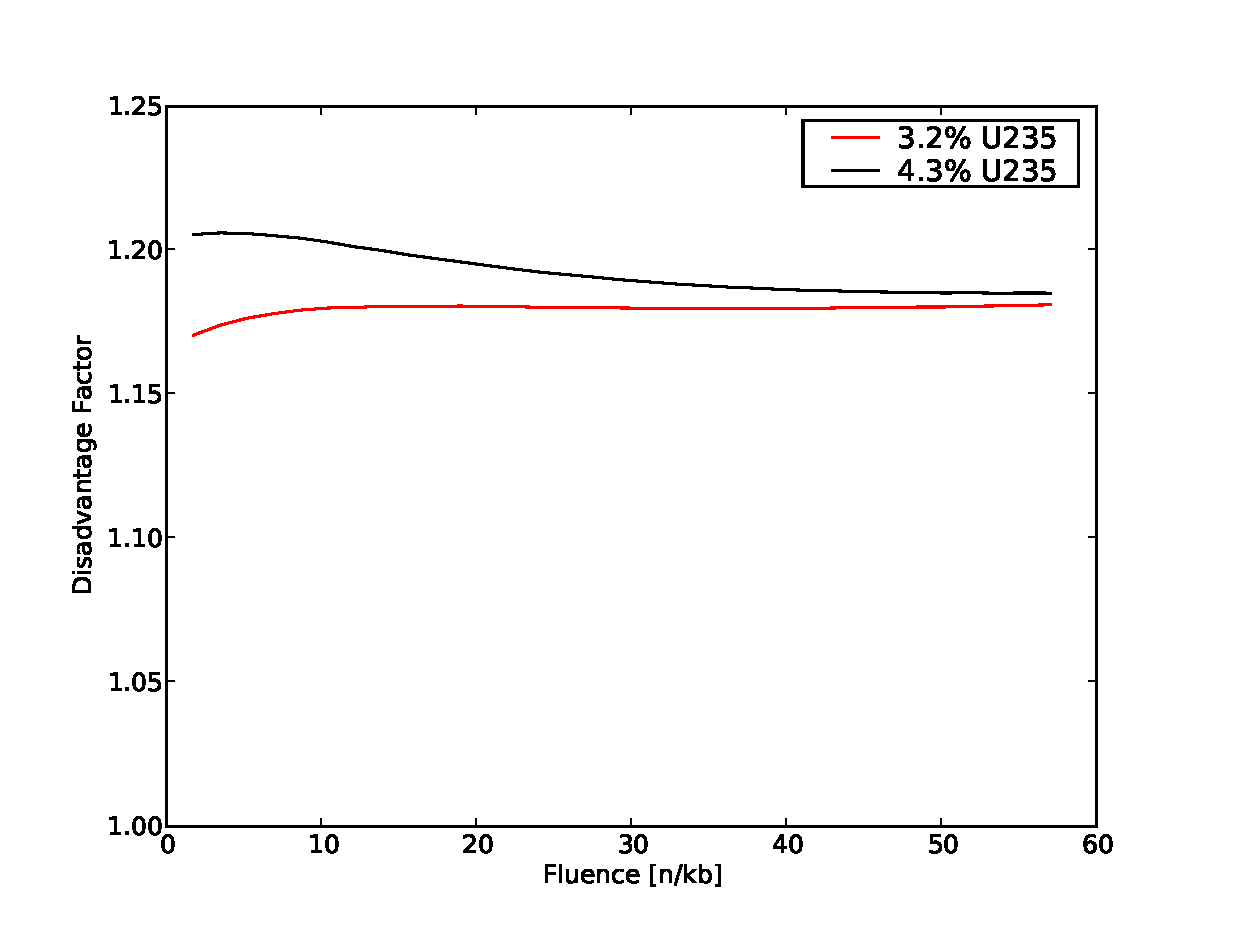
\includegraphics[scale=0.5]{one_group_method/figs/Fig04.eps}
\end{center}
\end{figure}
Thus the coolant destruction rate is then given as
\begin{equation}
\label{1g_dC_F}
d^C(F) = \zeta(F) \cdot \sum_i m_i^C \cdot d_i(F)
\end{equation}
Note that the volumetric weight in $m_i^C$ for the coolant region already includes both 
empty and filled fuel pin slots.  Therefore the full-core destruction rate $D(F)$ is given by 
the sum of the destruction rate in the fuel and the destruction rate in the coolant.  Namely, 
\begin{equation}
\label{1g_D_F}
D(F) = d^F(F) + d^C(F)
\end{equation}
Now that $P(F)$ and $D(F)$ are known, $k(F)$ may be calculated as per equation \ref{1g_k_F}.  
Once again, $F\mbox{d}$ is defined such that $k(F\mbox{d}) = 1$ which yields the maximum discharge 
burnup $\mbox{BU}(F\mbox{d}) = \mbox{BUd}$.




\subsubsection{Multiple Batch Cores}
\index{Multiple Batch Cores@\emph{Multiple Batch Cores}}
\label{1g_sec:batch_ave}
What has just been shown is how to find the discharge burnup with a given fuel composition for a one
batch system.  However, for multiple batches of fuel the process is less straightforward as the 
production and destruction rates are averaged over their end of cycle values for each batch.  
The general idea is to perform these operations in reverse and then iterate over them.  
In other words, one picks a burnup and then solves for the multiplication factor.  Then one picks 
another burnup that will yield a $k$ closer to one and solves again for $k$.  This process continues 
until a $k$ is found that is acceptably close to one.  

The bisection method is preferred to pick successively closer values of $k$.  It is not prone to the 
erratic behavior that arises when Newton's method is used with pointwise data.   Furthermore, the 
bisection method ensures that the fuel is burnable.  To use the bisection method here there must 
be both some fluence where $k < 1$ and some fluence where $1 < k$.  Since the multiplication factor 
is in reality continuous and more or less monotonic, these conditions imply that at some fluence $k = 1$.  
However, if these conditions fail then the fuel has too little fissile material to sustain a chain reaction. 

\begin{figure}[htbp]
\caption{Burnup as a Function of Fluence for Sample LWR Fuel}
\label{1g_fig05}
\begin{center}
\includegraphics[scale=0.5]{one_group_method/figs/Fig05.eps}
\end{center}
\end{figure}

\begin{figure}[htbp]
\caption{The Multiplication Factor as a Function of Fluence for Sample LWR Fuel}
\label{1g_fig06}
\begin{center}
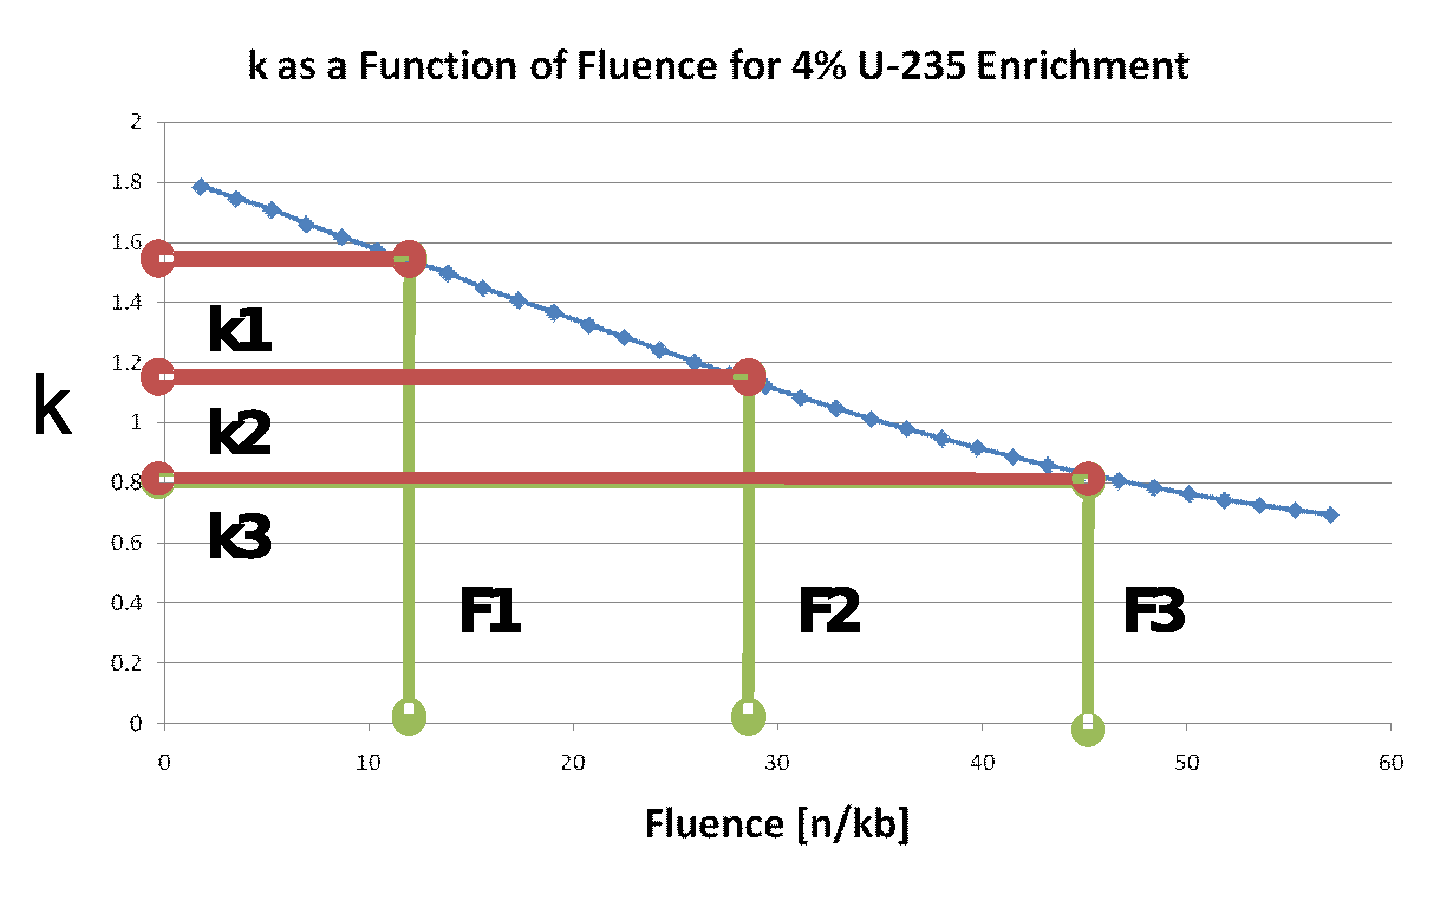
\includegraphics[scale=0.5]{one_group_method/figs/Fig06.eps}
\end{center}
\end{figure}

A walkthrough of the details of this process for multiple batches follows.  First, a maximum 
discharge burnup BUd is guessed.  Say without loss of generality that the system at hand is 
concerned with a three batch refueling cycle.  Then, assuming equal interbatch power sharing, 
the fluence must be found for three burnups, namely BUd, 2/3 BUd, and 1/3 BUd.   Lines drawn on 
Figure \ref{1g_fig05} from the burnup axis to the curve and then down from the curve to the fluence 
axis will give the fluence at the three points required.  Note that the highest fluence ($F3$ here) 
is the fluence at discharge $F\mbox{d}$.  After the fluence for each of the burnups has been calculated, 
the multiplication factor of the system needs to be known. 

To achieve this for a multibatch core, a flux-weighted batch averaging procedure is followed.  
The multiplication factor at each fluence is determined by the $P(F)/D(F)$ ratio.  Denote the batch 
number that a parameter is associated with by the index subscript ``b''.  In Figure \ref{1g_fig06}, 
the three $k_b$s correspond to the three fluences chosen and here $k_b(F_b) = P_b(F_b)/D_b(F_b)$.  
These are interpreted as the multiplication factors if the full core was in fact composed entirely 
of fuel that had been exposed to this fluence. Thus the true multiplication factor of the core is 
the weighted average of the production divided by destruction rates with the flux as a weight for 
``B'' number of batches.
\begin{equation}
\label{1g_k_batch_ave}
k = \frac{\sum_b^B \frac{P_b(F_b)}{D_b(F_b)} \phi_b}{\sum_b^B \phi_b}
\end{equation}
However, the flux $\phi_b$ in equation \ref{1g_k_batch_ave}, the average flux within batch $b$, is not known.  
Thus because the batch power remains constant $\phi_b$ does not.  Yet the flux is by definition the time 
derivative of the fluence. Thus a good approximation of the flux is given in equation \ref{1g_k_batch_ave}.
\begin{equation}
\label{1g_phi_b}
\phi_b \approx \frac{\Delta F}{\Delta t}
\end{equation}
Here, $\Delta F$ can be measured at a given fluence by perturbing $\mbox{BU}(F)$ by a small amount 
and finding the $\Delta\mbox{BU}$.  This is easily done as $\Delta\mbox{BU}/\Delta F$ is identically 
the slope of the $\mbox{BU}(F)$ graph at fluence $F$ as seen in Figure \ref{1g_fig05}.  Given the 
assumption of constant power density, a change in burnup yields a corresponding change in time such that
\begin{equation}
\label{1g_delta_t}
\Delta t = \Delta\mbox{BU} \cdot \frac{T_{\mbox{res}}}{\mbox{BUd}}
\end{equation}
Where BUd is the discharge burnup guess and $T_{\mbox{res}}$ [days] is the residence time that the 
fuel took to achieve this discharge burnup. Combining equations \ref{1g_phi_b} \& \ref{1g_delta_t}, 
$\phi_b$ is found to be
\begin{equation}
\label{1g_phi_b_1}
\phi_b \approx \frac{\Delta F}{\Delta \mbox{BU}} \cdot \frac{T_{\mbox{res}}}{\mbox{BUd}}
\end{equation}
Inserting equation \ref{1g_phi_b_1} into equation \ref{1g_k_batch_ave} an expression for the effective 
multiplication factor for a multiple batch system at the time that a batch is discharged is obtained.
\begin{equation}
\label{1g_k_batch_ave_1}
k \approx \frac{\sum_b^B \frac{P_b(F_b)}{D_b(F_b)} \cdot \left. \frac{\Delta F}{\Delta \mbox{BU}} \right|_b \cdot \frac{T_{\mbox{res}}}{\mbox{BUd}}}
                {\sum_b^B \left. \frac{\Delta F}{\Delta \mbox{BU}} \right|_b \cdot \frac{T_{\mbox{res}}}{\mbox{BUd}}}
 =  \frac{\sum_b^B \frac{P_b(F_b)}{D_b(F_b)} \cdot \left. \frac{\Delta F}{\Delta \mbox{BU}} \right|_b }
                {\sum_b^B \left. \frac{\Delta F}{\Delta \mbox{BU}} \right|_b}
\end{equation}
Now that a $k$ has been found, its value is converged to unity via the bisection iterations.  Another 
value of the maximum discharge burnup is then chosen and this process is repeated until a BUd is found 
that yields a $k = 1$.  Figures \ref{1g_fig05} \& \ref{1g_fig06} represent the process of finding a 
multiplication factor for a sample three batch system for a light-water reactor core.  

In the process of determining the maximum discharge burnup $F\mbox{d}$ is also found.  It is also 
easy to perform a mass-weighted linear combination of the isotopic transformation matrices. From here 
how each isotope initially present is transmuted at any fluence is known.  The mass of the j\superscript{th} 
nuclide at fluence $F$ is called $M_j(F)$ [kg\subscript{j}/kgIHM] and is given by
\begin{equation}
\label{1g_trans_Mj}
M_j(F) = \sum_i m_i^F \cdot T_{ij}(F)
\end{equation}
Here ``i'' represents isotopes initially present in the fuel.  Plugging in the fluence at discharge 
$F\mbox{d}$ into equation \ref{1g_trans_Mj} will yield the mass of isotope ``j'' in the spent fuel per 
kilogram of IHM.  Performing this operation for all ``j'' isotopes of interest will yield the isotopic 
output vector for the core.  Since fission product masses were included in the transformation matrices, 
the fission products at discharge are also known.  

\begin{figure}[htbp]
\caption{$M_j(F)$ for a Sample Fast Reactor for a Variety of Species}
\label{1g_fig07}
\begin{center}
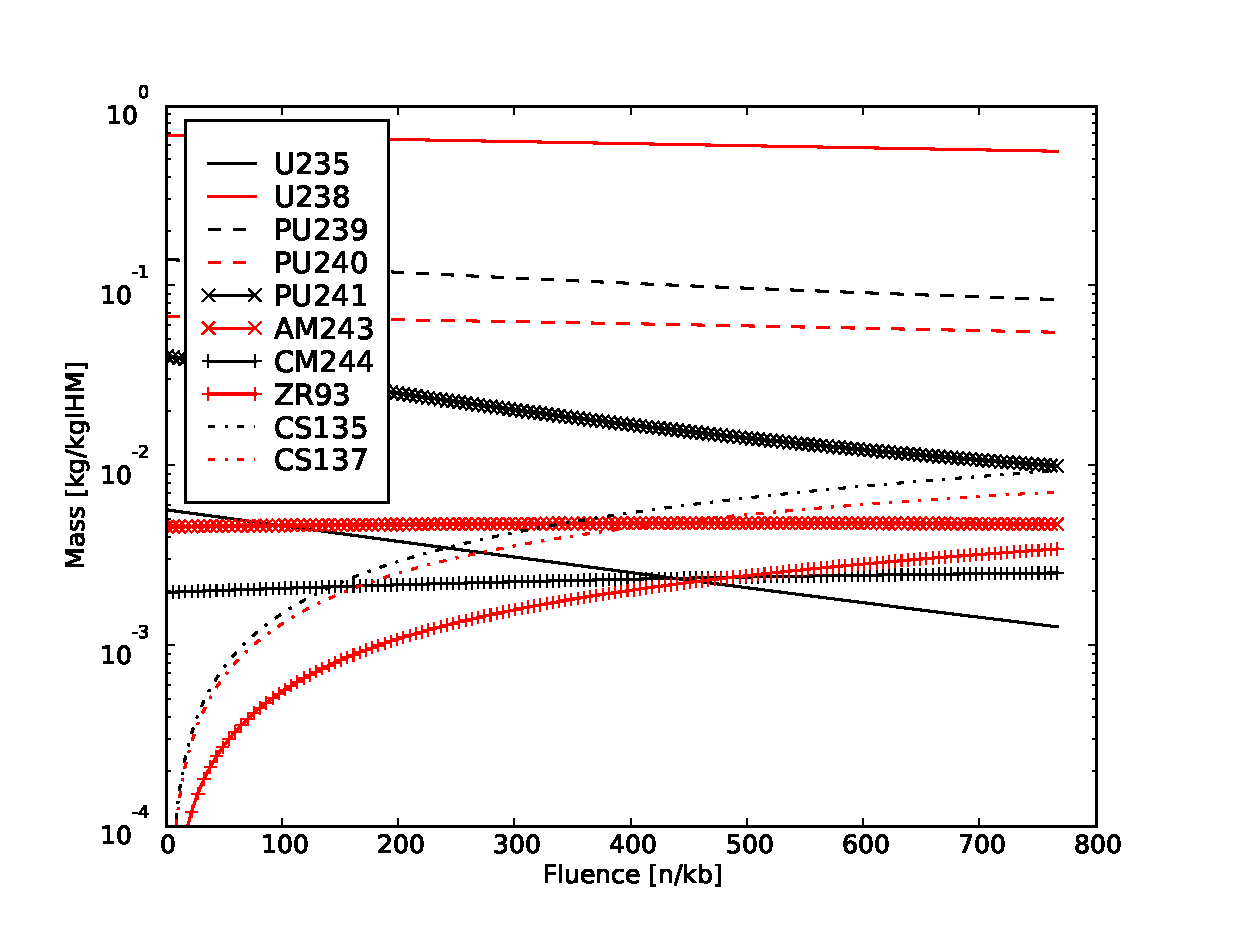
\includegraphics[scale=0.5]{one_group_method/figs/Fig07.eps}
\end{center}
\end{figure}

Figure \ref{1g_fig07} shows a graphical representation of the $M_j(F)$ for various isotopes present 
in a fast reactor.  Each curve for each nuclide is the superposition of all of the transformation 
matrices with their weight, as described above.  Some species, such as \nuc{U}{238} and \nuc{Pu}{239}, 
are burned out of the core faster than they are bred back in and are therefore represented by lines of 
negative slope.  Other isotopes, namely fission products, were not initially present and get bred into 
the core by any fissioning species.  These are shown as the curves growing towards some asymptote.  
Still other nuclides, higher order species like \nuc{Am}{243} and \nuc{Cm}{244}, have a more dynamic effect.  
They grow into the core and then peak and start to burn out.  

In conclusion, the above is an algorithm for finding the maximum discharge burnup and its discharge 
composition given only a fuel form represented by mi, the pre-generated burnup parameters ($p_i(F)$, 
$d_i(F)$, $\mbox{BU}_i(F)$, and $T_{ij}(F)$), the number of batches in the core $B$, and the non-leakage 
probability $P_{NL}$.  However, methods for generating these burnup parameters have not been discussed.  
This follows in the next section. 



\subsection{Generating Burnup Parameters}
\index{Generating Burnup Parameters@\emph{Generating Burnup Parameters}}
\label{1g_sec:gen_BU_param}
The burnup parameters $p_i(F)$, $d_i(F)$, $\mbox{BU}_i(F)$, and $T_{ij}(F)$ are typically calculated 
for a specific reactor design.  However, if the reactor type is perceived as being representative of 
all reactors of that type then the burnup parameters may be applied generally to all reactors of this 
type without having to recalculate new $p_i(F)$, $d_i(F)$, $\mbox{BU}_i(F)$, and $T_{ij}(F)$.  
Qualitatively, what it means to be representative of a reactor type and fuel composition is that the 
neutron energy spectrum inherent in the few-group cross sections used to generate the burnup parameters 
is similar to that of other reactors of this type and other fuel compositions that will be studied.   

In this study, the burnup parameters are calculated and tabulated based on the reactor-specific data 
libraries created from ORIGEN 2.2 [7] isotope-by-isotope burnup analyses.  As mentioned, the ORIGEN 
input libraries contain cross sections that are thought of as generic to a reactor type and range of 
fuel compositions.  For example, the libraries used here for fast reactors were prepared for a sodium 
cooled burner reactor with a target conversion ratio of 0.5.  This reactor is described in more detail 
in [4].  The burnup model therefore utilizes pre-computed libraries of the $p_i(F)$, $d_i(F)$, 
$\mbox{BU}_i(F)$, and $T_{ij}(F)$ that were built up from ORIGEN runs.  These libraries contain point 
wise data as a function of fluence.  Recall that all data in these libraries track the evolution of the 
parameter on a per unit mass basis.

To be more explicit, ORIGEN 2.2 is run for a kilogram mass of a given nuclide with the characteristic 
ORIGEN libraries.  Therefore, the isotopic mass balances and reaction rates obtained from this run 
reflect the evolution of one kilogram of this isotope within the core.  The ORIGEN output is then 
parsed and placed in the appropriate libraries for usage by the burnup model.  These ORIGEN runs are 
performed for all nuclides in the core.  Naturally, if one were to use initial ORIGEN libraries for a 
different reactor type, then the tables and matrices generated here would be representative of this 
other reactor.  These libraries only need to be generated once ever for a given reactor type, geometry 
and representative fuel composition.

In addition, the representative cycle-average neutron energy spectrum changes with BUd.  This is because 
more fissile fuel is needed to achieve increased burnups and even for an identical fuel to coolant volume 
ratio the spectral dependence on burnup is often too large to neglect.  Thus for thermal-spectrum systems 
ORIGEN input libraries are prepared for a number of differing BUds: for PWRs, for instance, libraries 
representative of 20, 33 and 50 MWd/kgIHM discharge burnups have been used in these studies.  Thes 
libraries are interpolated to create customized libraries at any burnup in this range.  They thus 
capture the dependence of the cycle-average cross sections on discharge fluence and, implicitly, 
initial isotopics.  This is of more significance to PWRs as fast reactor spectra are relatively more 
stable; moreover, to investigate high-burnup PWR fuels additional libraries for BUd of 70 and 100 MWd/kgIHM 
have been prepared using assumed initial \nuc{U}{235} enrichments of 5.5 and 8 w/o, respectively.

Even systems whose spectra are less sensitive to initial composition and burnup must be treated using a 
number of cross section libraries prepared from detailed transport calculations.  For the sodium-cooled 
FR design studied here, for example, a number of libraries are available.  The core aspect ratio for the 
design varies to ensure acceptable coolant void reactivity properties as the conversion ratio and uranium 
content decrease, so distinct sets of libraries were prepared for 0.5 (used in this study) and 0.25 target 
conversion ratio designs.  Additionally, separate libraries were prepared at each conversion ratio for 
fuels with higher and lower minor actinide (MA) content.   The higher MA case is representative of the 
feed to a FR if Pu from spent UOX is first burned in MOX, while the lower MA library, the one used in 
this study, reflects the TRU content with no MOX burn.



\subsubsection{Hydrogen Cross Section Rescaling}
\index{Hydrogen Cross Section Rescaling@\emph{Hydrogen Cross Section Rescaling}}
\label{1g_sec:H_rescale}
The one group cross sections are functions of fuel burnup and therefore fluence, in some cases quite 
strongly so.  The model supports the adjustment of cross sections \nuc{H}{1} and therefore production 
and destruction rates as well as transmutation rates \nuc{H}{1} with fluence.  For instance, the effective 
one group radiative capture cross section of 1H in typical PWR coolant changes significantly with fluence 
as the flux spectrum in the core evolves to maintain constant power density.  Just as with the interpolation 
of the ORIGEN input libraries, the hydrogen cross section may be parameterized around the burnup that the core 
has experienced.  Moreover, hydrogen contributes about 10\% to the total destruction rate in the core.  
Thus a significant change in the hydrogen cross section could yield an appreciable error in the model as 
formulated above.  What follows is more of an adjustment to the hydrogen one-group cross section than a 
true mutli-group theory response.  However, this provides an easy to calculate and integrate model to 
reduce the error induced into the neutron destruction rates.

To account for these spectral variations an f-factor is introduced that is a function of the burnup 
$\mbox{BU}(F)$.    $f(F)$ is a unitless factor by which all hydrogen destruction rates $d_H(F)$ are 
multiplied by in equations \ref{1g_dF_F}-\ref{1g_D_F}. Two hydrogen cross sections are known for two 
burnups.  These were taken from the ORIGEN cross section libraries prepared for 33 and 50 MWd/kgIHM 
burnups in PWRs.

Thus $f(F)$ is the computed by drawing the line between these two points and dividing it by the cross 
section that was used for the ORIGEN runs.  Since ORIGEN was run using the 33 MWd/kgIHM library, the 
line is simply divided by 0.03474 barns.  The equation for $f(F)$ is therefore, 
\begin{equation}
\label{1g_f_F}
f(F) = 1.36927 - 0.01119 \cdot \mbox{BU}(F)
\end{equation}
As is seen in this extrapolation, the per atom hydrogen neutron destruction rate can vary considerably.  
Multiplying $f(F)$ by $d_H(F)$ results in an increase of the accuracy of all destruction rate and 
multiplication factor data that is computed.  The inclusion of the hydrogen rescaling factor and 
subsequent effects on BUd and initial compositions will be discussed in a later section with regards 
to the example of standard PWRs.  



\section{Fuel Cycles}
\index{Fuel Cycles@\emph{Fuel Cycles}}
\label{1g_sec:fc}
The Global Nuclear Energy Partnership (GNEP) plan for domestic fuel cycles offers many possible 
pathways.  With most of these options GNEP hopes to reduce the stockpile of United States 
transuranics (TRU) and obviate the technical need for a second repository during this century.  
Separated transuranics are moreover seen as dangerous to nuclear non-proliferation goals.  
Furthermore, most TRU species negatively impact repository performance as compared to an equivalent 
mass of NU.  Two fuel cycles involving recycle - uranium recycle in PWRs and full TRU recycle in 
FRs - are examined here as case studies to which the method presented above is applied. 


\subsection{Uranium Recycle Fuel Cycle}
\index{Uranium Recycle Fuel Cycle@\emph{Uranium Recycle Fuel Cycle}}
\label{1g_sec:UFC}
The first of the fuel cycles that are analyzed here explores blending of RU with enriched NU to 
achieve sustained uranium recycle in light water reactors (LWR).  Since RU is a product of 
reprocessing of light water reactor spent nuclear fuel (LWR SNF), the front end for the RU creation 
process includes the back end of the reprocessing based LWR-NU fuel cycle.  The application of the 
burnup model to the RU burning reactor will be demonstrated through the study of this fuel cycle.

Figure \ref{1g_fig08} depicts the RU blending option studied here.  Red arrows in Figure \ref{1g_fig08} 
connote RU flow stemming from the UREX+ reprocessing component or the enrichment component.  Black arrows 
that lead out of components indicate flows that do not comprise the mass input streams to the RU burning reactor.  
\begin{figure}[htbp]
\caption{RU Fuel Cycle}
\label{1g_fig08}
\begin{center}
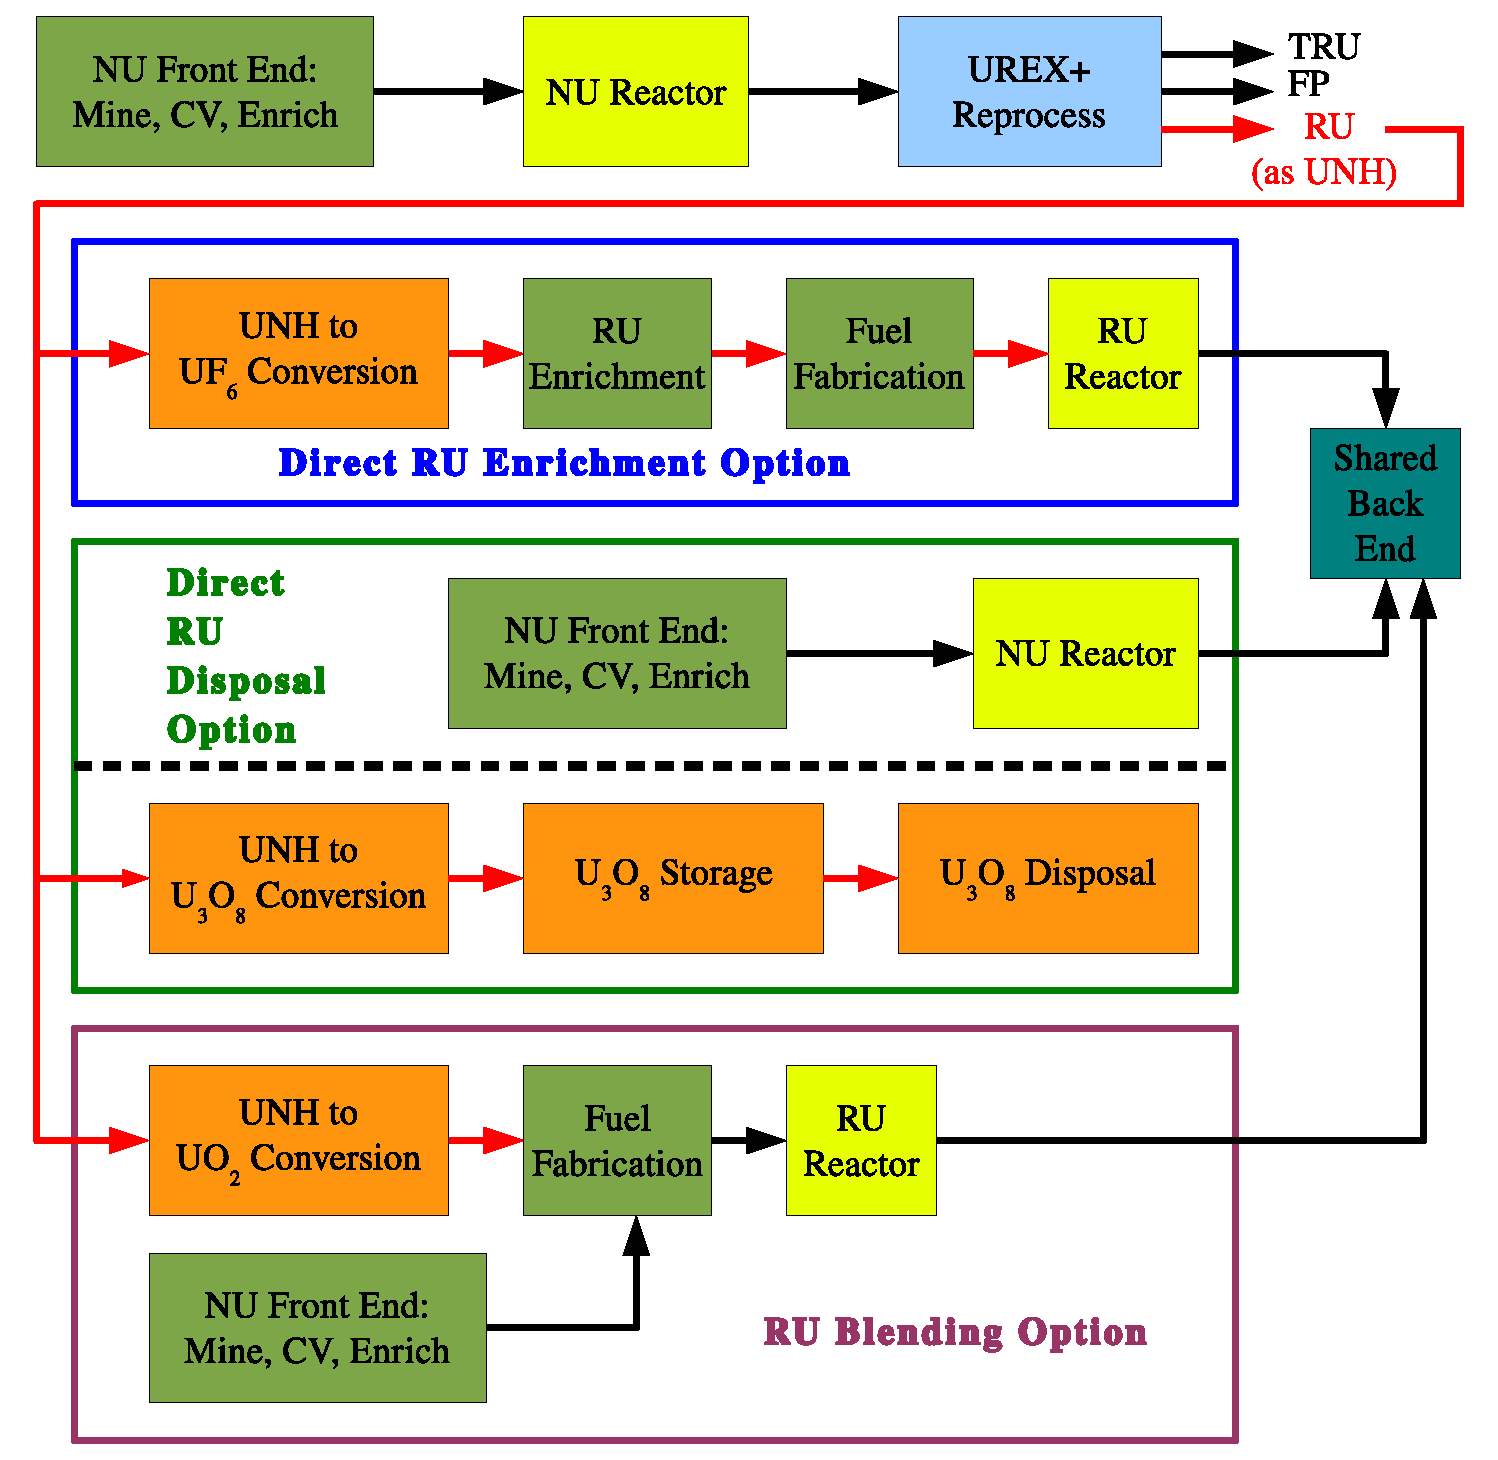
\includegraphics[scale=0.5]{one_group_method/figs/Fig08.eps}
\end{center}
\end{figure}
Blending RU with enriched natural uranium is a method of increasing the fissile content of the RU while 
also impeding the buildup of \nuc{U}{236}, a neutron poison.  From the standpoint of the fuel cycle material 
balance alone, if the utilization of RU is to be maximized the best material to serve as a blend stock with 
RU is highly enriched uranium (HEU).  HEU is in limited supply as a blend stock [8] and its use for civilian 
applications is undesirable; therefore, if this strategy is to be sustained, the blend stock would be low 
enriched uranium (LEU).  

LWR SNF contains a higher enrichment of \nuc{U}{235} than NU; therefore RU blending may be economically 
advantageous over the once-through fuel cycle given that reprocessing is already taking place to recover 
TRU. The weight percent of \nuc{U}{235} in the legacy spent fuel of the United States is between 0.8-0.9\% [6].  
However, LWR SNF also has had \nuc{U}{236} bred into it in non-negligible amounts of around 0.3-0.5\%.  
As \nuc{U}{236} is a neutron poison, the advantage of the extra \nuc{U}{235} in RU is not immediately 
quantitatively obvious.  Therefore, to increase the fissile content of an RU fuel form, it is blended 
with LEU. This LEU blend stock serves to dilute the \nuc{U}{236} and thereby decrease its negative 
impact on the neutron balance in the core. 

Fuel that goes into the RU reactor must be assigned a target burnup; for reasons of simplicity and 
practicality, it will be assumed that it is desirable to achieve parity between the traditional LEU- and 
RU-bearing fuel burnups.  Since the RU isotopic composition is set by the burnup in the initial reactor, 
the free parameters that are used to match the burnup of RU fuel to that of virgin LEU fuel in the reactor 
are the LEU enrichment and its mass fraction in the blended LEU-RU stream.    

The first blending option is that the mass of LEU blend stock per unit mass of RU is held constant.  
Thus the fissile content of the RU-bearing fuel is controlled by the enrichment of the LEU.  On the 
other hand, the LEU enrichment can be held constant and the mass that is mixed with the RU may be 
varied.  In this second case the LEU enrichment may be up to 19.9\%.  

It should be noted that higher LEU enrichment levels mean that more RU can be blended for a given 
mass of LEU.  But generally, near-future enrichment plants will not be licensed to produce LEU at 
greater than 8\% \nuc{U}{235} enrichment. However, the LEU/HEU limit is 19.9\% so it is conceivable 
that if RU recycle came to fruition civilian enrichment facilities would be allowed to produce 19.9\% 
enriched product.  



\subsection{Fast Burner Reactor Fuel Cycle}
\index{Fast Burner Reactor Fuel Cycle@\emph{Fast Burner Reactor Fuel Cycle}}
\label{1g_sec:}
A fuel cycle that features full, sustained TRU recycle is the second one being examined.  The basis of the model used here is a fast reactor (FR) with LWR SNF top up.  The purpose of this fuel cycle option is to reduce the global actinide inventory per unit energy as compared to the standard once-through fuel cycle, with the specific aim of reducing transuranics.   To this end, the FR conversion ratio (CR) is less than unity.  The nominal value for the conversion ratio in this study is taken to be 0.5, consistent with the baseline sodium-cooled fast transmuting reactor point design used in GNEP scoping studies [2].  
(Scopatz, Schneider, Fig. 9)
Figure 9 depicts the FR fuel cycle that is being studied.  Once again, mass flows represented in red are the four mass streams that form the FR fresh fuel blend stock.  The mass of each stream relative to the others may be varied by the burnup model to achieve a target burnup.  The mass flows in black are the flows that are considered static to the burnup model and are not changed, though they may vary with fuel cycle pass number.  
Moreover because of the dynamic nature of the burnup model, the discharge burnup is not fixed but rather a target BUd is set as a parameter within the model.  Alteration of the BUd will change the balance of the FR input mass streams as well as all dependent isotopics.  However, burnup values of 51 MWd/kg for the LWR and 170 MWd/kg for the FR are used unless otherwise stated.  Both of these values were taken from the VISION [1] specifications for nominal LWR and FR cases.  Similarly, spent fuel from both the LWRs and FRs is allowed to cool for a time before being reprocessed.  The time that spent fuel of any sort is allowed to cool also affects the isotopics and mass stream material balances.  But once again, the cooling time is a parameter that may be specified within the fuel cycle model for which nominal values were taken here.
The input mass to the fast reactor is made up of four independent streams: the uranium coming from light water reactors (LWR-U), the transuranics coming from light water reactors (LWR-TRU), the uranium coming from fast reactors (FR-U), the transuranics coming from fast reactors (FR-TRU).  These streams are separated in the reprocessing facilities and then combined to form the input stream to the fast reactor.  The fission products from these streams are also removed from the fuel at this point and sent off to a disposal facility.  
It should be noted here that the reprocessing facility that deals with the light water reactor spent nuclear fuel (LWR SNF) and the reprocessing facility that handles the fast reactor spent nuclear fuel (FR SNF) are not the same.  They are displayed as one box in fuel cycle Figure 8 for ease of reading, although it is likely that these two fuel cycle components would be collocated.
Lastly, Figure 9 represents a closed fuel cycle which implies that actinides may be recycled indefinitely or until they are eventually burned as long as there exist enough FRs to handle the mass throughput.  Of course this is not strictly true since no separation process is perfect.  Some small actinide mass will be mixed with the fission products after reprocessing and be sent to the repository.  It is known that the reprocessing separation efficiencies ultimately affect repository performance [11].  However, because the isotopics change with every pass of TRU through the fuel cycle, there arises a mass stream feedback between the reactor burnup, the cooling time, and the reprocessing efficiencies that the burnup model handles with ease. 
The implication of a closed or partially closed fuel cycle is that mass may be sent through many recycles.  For a specific target FR burnup and other fuel cycle parameters, the relative masses and the isotopics of the four mass streams (LWR-U, LWR-TRU, FR-U, FR-TRU) may change significantly as a function of pass number.  However, one would eventually expect that equilibrium values for the mass balances and isotopics will be reached and indeed they typically are.  For some species, though, so-called equilibrium is not reached even after many recycles; indeed, in practice many decades, even centuries, would elapse before an ‘equilibrium’ scenario result would reflect reality.  Therefore, equilibrium fuel cycle simulation results must be interpreted with caution.  When equilibrium is achieved and how it is defined is discussed further in a later section.  



\subsection{Cooling Model}
\index{Cooling Model@\emph{Cooling Model}}
\label{1g_sec:cool_model}
Before reprocessing occurs, light water reactor spent nuclear fuel (LWR SNF) and fast reactor spent nuclear fuel (FR SNF) are typically stored and cooled.  This process represents the “Storage” boxes in fuel cycle Figures 8 and 9.  The cooling model computes the analytical solutions to the Bateman equations [12]: 
        (18)
Here, tC [years] is the time that the SNF spends in storage cooling,  Ni(tC) [kg] is the mass of the ith daughter of the parent species with mass N1 [kg]. The λs [1/years] are the decay constants for the respective nuclides in the decay chain.   The γs are the branch ratios that correspond to each decay constant for this decay chain.  
Finally, these results are sent to the reprocessing model (where separation efficiencies are applied), output parameters are recorded, graphs are generated, and (for the FR case) the next cycle starts.   It is therefore time for the dynamic fuel cycle results to be computed using the burnup model.





\section{The Fuel Cycle Model: Benchmarking \& Results}
\index{The Fuel Cycle Model: Benchmarking \& Results@\emph{The Fuel Cycle Model: Benchmarking \& Results}}
\label{1g_sec:fcmodel_benchmark}
The fuel cycle model is the computational wrapper that executes much of the calculation and analysis.  The fuel cycles that are studied are specified by a large set of inputs extending to the various intrinsic parameters of the reactors that comprise it.  For example, the PNL of the different reactors are specific to that reactor’s design and neutron transport characteristics.  Other parameters include the reactor’s target burnup, the amount of time that SNF spends in storage cooling, and the fuel cell specifications that are used.  Values for these parameters that were used in this study are presented in Table 1.  Knowing this information, the fuel cycle model wraps around the reactor burnup model and invokes it when input streams need to be mixed or spent fuel compositions must be found.  The fuel cycle model then sends the results of the burnup model to the next fuel cycle component (as seen in Figures 8 and 9).  Thus the fuel cycle model coupled with the burnup model developed here to produce unique, physics-based values for the material balances and isotopics for one or many recycle passes.  This represents an advantage over recipe based simulations which are not able to alter any of the input parameters at will whereas here all of them are allowed to change. 
(Scopatz, Schneider, Table 1)
It is important to point out that the burnup model is sensitive to the input parameters specified in Table 1.  To select the non-leakage probability PNL and calibrate the model, enrichment and burnup combinations were taken from VISION [1] libraries for LEU for a 3 batch core.  By thinly varying PNL and the coolant density ρC [g/cm3] and toggling the f-factor correlating cycle-average hydrogen cross sections with discharge burnup a wide range of values for enrichment for given burnups was generated.  These are presented in Table 2 along with benchmark enrichment/burnup values taken from two other sources.  The parameter set H was the one that was chosen for the actual model as it most closely represents reality and the VISION targets.  Note that the enrichment is in weight percent 235U and BUd is in units of [MWd/kgIHM].  This calibration must be carried out for each reactor system to be analyzed.
(Scopatz, Schneider, Table 2)
A series of benchmarks were carried out to verify both the fresh fuel composition and fuel burnup calculations.  The OECD Burnup Credit Criticality Benchmark [3] series is a composite of many international studies using independent, high fidelity neutronics codes acting on the same specifications.  The study selected for benchmarking, Phase I for PWRs, uses an initial fuel vector (3.6 w/o 235U with trace amounts of 234U and 236U) that is burned to 40 MWd/kg.  The study lists output isotopics at various stages during the burn and post-removal cooling.  
To benchmark the burnup algorithm developed here, the initial fuel vector and burn parameters are taken from the study but “generic” PWR cross section sets were used.  In other words, the cross sections developed for a reference 17x17 PWR lattice were used with the burnup model and detailed transport calculations to create customized cross section sets for the benchmark case were not carried out.  This situation reflects the procedure that might actually be carried in a fuel cycle scoping calculation, where it is desirable to treat all reactors of a single general type as represented by a generic archetype.  Table 3 compares the computed isotopics to the isotopic vector reported in the OECD study for a 40 MWd/kgIHM burn with no cooling.  The table also shows the standard deviation of the collected results for the 21 participants in the Phase-IB study.  
(Scopatz, Schneider, Table 3)
All values are given in terms of weight percent of initial heavy metal.    These results show that the present method matches the Burnup Credit within two standard deviations for most actinides.  The only species showing a much larger relative departure is 241Am.  241Am is formed almost exclusively thorugh 241Pu decay and there are two reasons for this departure.  First, the fluence-dependent isotopic transformation matrices were assembled using a constant flux 4x1014 [n/cm2/s] that is representative of most PWRs.  If the average flux and power density are somewhat lower, and hence the irradiation time is somewhat longer as is the case here, the model will under predict the 241Am buildup in the core.   Second, the model does not explicitly treat refueling downtimes when transmutation ceases but decay continues. Note that the deviation in long-term 241Am content is smaller because the concentration of the much more abundant parent, 241Pu, is reasonably accurate. 
It is also necessary to benchmark the feed stream blending and discharge burnup calculations.  This is best achieved in the context of a comparison of a fuel cycle material balance.  Material balances of this type generated using the high-fidelity material balance simulation package COSI [14] are available in a number of OECD systems studies, e.g. [15].  A benchmark of the equilibrium material balance for a PWR/FR fleet has been carried out.  In this benchmark, the methodology described here is used to find the enrichment of PWR fuel to achieve a specified burnup as well as to derive the equilibrium FR fresh and spent fuel compositions through the cycle iteration procedure described in this paper.  Specific results benchmarked included the PWR/FR thermal power split, the isotopic composition of the burned fuel, and the fuel cycle cost derived from the material balance flowsheets.  A detailed description of the benchmark results may be found in section 3.2 of the companion paper [13] appearing in this issue.  Since the benchmark fuel cycle scenario served as a point of departure for the system study presented in that paper, and also because items outside the scope of this paper such as cost calculations were being benchmarked, it was felt more appropriate that this benchmark be presented there.





\subsection{The Recyclable Uranium Fuel Cycle}
\index{The Recyclable Uranium Fuel Cycle@\emph{The Recyclable Uranium Fuel Cycle}}
\label{1g_sec:RUFC}
The RU fuel cycle described here does not preclude multi-recycle of transuranics; instead it focuses only upon the uranium component of an integrated recycle strategy.  Moreover, for purposes of illustration only the first uranium recycle pass is considered.  A second example applying the burnup model to a dynamic case will be covered in the FR fuel cycle section.
To further characterize what is happening in the burnup model, it is of interest to characterize the isotopic breakdown of the neutron production and destruction rates in the core.  To do so, one simple case is considered.
For this illustrative case the 235U enrichment is chosen at 4.0%, while the 236U enrichment is set to 1.5%.  Three batch fuel management is assumed and a graph of BU(F) is made in analogy to Figure 5.  The discharge burnup BUd of this fuel is not known a priori but it is instead calculated via the burnup model that was described above.  BUd here turns out to be approximately 37 MWd/kgIHM.  Figures 10, 11, 12, and 13 show the computed core-average neutron production and destruction rates for burnups of 0, 1/3 BUd, 2/3 BUd, and BUd.  Zero burnup here indicates the neutron production and destruction rates for fresh fuel that has just been loaded into the reactor.  
It is crucial to note that the species-specific production and destruction rates shown in these figures reflect the isotope and all of its daughters.  For example, by the end of life, most of the neutrons are coming from 238U and its daughters.  In fact very few neutrons are spawned from 238U itself, but rather from its daughter 239Pu.  Similarly, by the time the fuel has reached BUd much of the 235U has already burned off.  These figures show that the neutron balance is well represented by a mass-weighted linear combination of initial isotopics; therefore the fluence dependent balance depends strongly on initial composition of the fuel.  To scope the merit of RU blending strategies, It has been found to be useful to parameterize discharge burnups of RU-bearing fuels around this dependence.
(Scopatz, Schneider, Fig. 10)
(Scopatz, Schneider, Fig. 11)
(Scopatz, Schneider, Fig. 12)
(Scopatz, Schneider, Fig. 13)
To accomplish this the achievable burnup is parameterized as a function of the fresh fuel initial 235U content, initial 236U content, and the number of batches in the fuel management scheme.    Note that given this small number of degrees of freedom, the whole parameter space may be comprehensively mapped.  Therefore the discharge burnup can be found as a function of these three variables (235U%, 236U%, B).  With the FRs, finding such a parameterization would be bulky and unwieldy if even computable.  Moreover, it would be prohibitive to try to do so for FRs since the parameter space of initial isotopes is larger by at least an order of magnitude.  
The functional form of the equation that gives BUd is shown in Equation 19.  In this equation, BUd is the discharge burnup achievable [MWd/kgIHM], x is the weight percent of 235U in the fresh fuel [(w/o)IHM], y is the weight percent of 236U in the fresh fuel [(w/o)IHM], and B is the number of batches.  All other letters appearing in Equation 19 are parameters of the fit and have units appropriate to their placement.  The values of these parameters that were obtained for the data set generated are given in Table 4.
        (19)
(Scopatz, Schneider, Table 4)
In Equation 19, fit parameters and the dependent variables are based on various physical meanings.  First, the 2B/(B+1) dependence of BUd comes directly from the results of a linear reactivity model with the core burnup being an independent variable when calculating the reactivity.  The proof of this dependence and its physicality are given in [10]. Moreover, the j(x-h)m term comes from the fact that the major trend for burnup follows a power law. One expects that the burnup would, as a function of fluence, asymptotically approach the maximum possible burnup (~935 MWd/kgIHM).  However, the power law, with “m”<1, seen here is a good approximation for the relatively low burnups achieved in PWRs. “j” scales this term up to the valid burnup range and “h” slides the burnup over to the 235U enrichment under which burning is not feasible.
Furthermore, at a given 235U enrichment, BUd is seen to have a near-linear dependence upon 236U content.  Because the 236U is a poison and is present in relatively small amounts, incremental changes in its enrichment yield matching changes in the burnup.  More explicitly, “s” determines how much a given 236U content affects the burnup.  Additionally, “s” is negative because 236U only destroys neutrons and does not directly increase the energy gained from the fuel per atom IHM.  However, BUd also decreases linearly with the 235U content.  The “tx” term is a correction factor to the power law term.  It slightly weights lower 235U enrichments preferentially to higher burnups.  This term exists because there is 236U present.  This term captures the poisoning effect of 236U: with increased 236U more 235U is needed to achieve a given burnup.  Lastly, the constant “k” term scales up the burnup to the appropriate base value.
Thus Equation 19 satisfies the requirements of fitting the maximum discharge burnup data to 235U content, 236U content, and the total number of batches while having a physical interpretation.  
Figures 14 and 15 show how the closed form equation with the given parameters fits to the actual data that was generated for three and six batch cores respectively.  These figures show that the fit with the data is quite good for 235U enrichments between 2 - 6% and 236U content from 0 - 4.5%.   Having such a fit equation is useful as it allows for the near instant calculation of the burnup for a PWR bearing RU fuel.  
There is a large advantage to this with respect to the RU fuel cycle.  Recall that the fuel cycle model mixes an RU stream from LWR SNF and an enriched NU stream.  Thus using Equation 19, the maximum achievable burnup of the mixed fuel can be found with ease and without resorting to a lengthy calculation or resubmitting the relevant data to the burnup model.  Moreover, given the 236U enrichment, the number of batches, and a target burnup, the fit equation can then be easily iterated to find the 235U enrichment required.  
(Scopatz, Schneider, Fig. 14)
(Scopatz, Schneider, Fig. 15)
In Figure 16 the 236U is held at a constant 1% while the number of batches is allowed to vary.  Note that in all three of these figures the low burnups do not fit as well to Equation 19. However, this region of discharge burnups of less than 20 MWd/kgIHM is of low concern for PWRs.   Moreover, as a function of batch number Equation 19 fits very well to all cases save the unlikely single batch case.  
(Scopatz, Schneider, Fig. 16)
Lastly, fuel cycle material balances may be expediently generated.   As an example case, set the target burnups of the RU- and NU-burning reactors to 51 MWd/kgIHM.  As discussed above, either the relative mass of RU/LEU or the LEU enrichment may be the free variable.  Allowing the LEU enrichment to be free and the mass of RU and LEU to be blended is the same,  Figure 17 shows the mass balance of the fuel cycle just defined and it can be seen that the LEU enrichment needed to obtain the target burnup for the blended fuel is 8.5%.  Note that this figure is in analogy to Figure 8, but with mass stream values included.  Moreover, Figure 17 is normalized to 1 kgIHM in the RU reactor.
(Scopatz, Schneider, Fig. 17)



\subsection{The Fast Reactor Fuel Cycle}
\index{The Fast Reactor Fuel Cycle@\emph{The Fast Reactor Fuel Cycle}}
\label{1g_sec:FRFC}
A walkthrough follows of how to apply the burnup model algorithm to the closed fast reactor system described above.  The first time a fast reactor system comes online, there exists no FR-U and FR-TRU streams from prior cycles so these mass flows and compositions are set to zero.   This leaves only reprocessed LWR-U and LWR-TRU streams to be mixed in order to obtain the burnup value specified for the fast reactor.  Luckily these two parameters in fact reduce to only one variable since LWR-U = 1 – LWR-TRU.  Therefore the system has only one degree of freedom.  
It should be noted here that the LWR-U and LWR-TRU internal isotopic compositions remain constant over all fuel cycle passes through the fast reactor.  This is because the LWR burnup remains the same  and identical LWR SNF is always used to top up the fast reactor.  
To obtain the LWR-U/LWR-TRU ratio that achieves the target burnup, an initial guess of the ratio is made.  This resulting fuel is then sent to the burnup model and maximum discharge burnup is calculated.  A root finding method is then used to iterate over the ratio and BUd until a proportion of LWR-U/LWR-TRU is found that generates the target burnup.  The bisection method is once again applied due to its usefulness with regards to pointwise approximations of continuous data.
More precisely, two initial conditions are first calculated for the bisection method to be used.  Firstly, a BUd is calculated (via the burnup model) for a fuel that is composed of entirely LWR-TRU.  If this is not a valid fuel form (as discussed above) then an incremental amount of LWR-U is added until a valid, burnable form is reached.  The second initial condition is just the inverse.  A BUd is found for a fuel that is primarily or all LWR-U.  These two conditions serve to bound the range of available burnups for the FR fresh fuel.  If the FR target burnup is outside of this range, then the remainder of the calculation is impossible.  Otherwise, the bisection method may be applied with these two starting conditions.  Upon reaching the target burnup, the amount of LWR-U and LWR-TRU that go into the fast reactor on the first pass of the FR fuel cycle is now known.
The isotopic output of this first fast reactor burn is then sent to the cooling model.   After the FR SNF has been decayed for the appropriate amount of time the reprocessing separation efficiencies are applied.  These separation efficiencies are set initially and are constant for the entire fuel cycle, although they may vary between individual chemical elements.  Fuel cycle parameters are now calculated and recorded.  This concludes the first cycle pass through the fast reactor.  
The second and further passes proceed similarly to the first.  However unlike in the first pass, the four mass streams (LWR-U, LWR-TRU, FR-U, and FR-TRU) now all exist as the FR-TRU and U discharged from the fast burner will be reloaded in the next cycle.  However, FRs convert 15-20% of their (initial actinide) mass into fission products over the course of their burn and considerable top-up from LWR-U and LWR-TRU will be required.  
However, the same problem remains as in the first pass case.  This that the LWR-U/LWR-TRU proportion that generates a burnup that equals the target burnup is not known a priori.  Thus the same strategy that was used in the first cycle is employed to find this proportion.  Once again, two guesses are made as to what the stream’s relative fractions are.  These bound the burnups available and the bisection method is applied to calculate the LWR-U/LWR-TRU ratio that hits the target burnup.  
Now that the target burnup has been reached and the fresh fuel burned, it becomes spent fuel once more.  The FR-SNF is again stored and cooled.  These results are then sent to the reprocessing code (where the separation efficiencies are applied).  Fuel cycle parameters that are specific to this pass are now calculated and stored.
This process may continue indefinitely as there are an infinite number of cycles possible.  However, fuel cycle parameters (such as isotopic concentrations in the fresh and spent fuels, uranium and transuranic masses) typically come to ‘equilibrium’ given enough passes through the system.  Two approaches to determining equilibrium status were considered: the stabilization of certain tracked isotopes or the convergence of the FR fresh fuel transuranic fraction.   This TRU fraction is tracked until it converges to within error, say a 1% change between the last cycle and the next-to-last cycle at which time equilibrium is declared.    The advantage of this method is that, for all practical applications, it ensures that the four input mass streams have all converged on their own and the gross mass balance is in near-equilibrium.  
If the fuel cycle study is concerned with the prevalence of isotopes having, for instance, a strong effect on repository performance it is wiser to develop a list of important species whose convergence is to be tracked.  Then at the start of each cycle after the first, the change of these isotopes concentrations in the spent fuel is calculated.  If all isotopes in the list have converged to within some allotted error (perhaps 1%), then the fuel cycle as a whole is said to have converged.   In the FR case considered here, 239Pu, 240Pu, and 242Pu dominate the TRU by mass and converge after only a few cycles.    Moreover, 242Pu is the precursor isotope for production of most of the trans-plutonium elements.    Even though other actinides affect the FR burnup, many either do so to a lesser degree or are present in such small amounts that they do not significantly impact the neutronics of the system.  However depending on the application being studied the convergence criteria may differ.  For instance, the radiologically significant isotope 244Cm still has not converged by the above definition, even after ten cycles.
Now that the entirety of the fuel cycle over multiple passes has been computed via the prior algorithm, a number of cycle specific parameters may be calculated.  The following example data was all produced using LWR SNF isotopic vectors from VISION [1]. Moreover the following table displays initial parameters input into the computational burnup and fuel cycle models.
(Scopatz, Schneider, Fig. 18)
The first set of parameters displayed is the input fractions of the four input mass streams into the fast reactor: LWR-U, LWR-TRU, FR-U, and FR-TRU.  This is shown in Figure 18.  The input mass of fuel into the fast reactor comes in some part from LWR spent fuel (1 kg or less) and partially from recycled FR fuel.  Note that all streams are normalized to 1 kgIHM for each cycle.  The LWR streams here are the parameters that are explicitly iterated over in the fuel cycle model in order to achieve the target FR burnup.  Note that the first cycle is comprised of only LWR spent fuel (as discussed above) and then these curves quickly level off.    Also recall that all FR actinide mass (sans what is decayed away in storage and what is lost in reprocessing) returns to the FR on the next pass.  Since the FR converts roughly 20% of its initial fuel to fission products, this explains why the sum of FR-U and FR-TRU levels off at about 0.8.  
(Scopatz, Schneider, Fig. 19)
Unlike the LWRs, the fast reactor output stream is also a function of cycle number.  Figure 19 plots the fraction of the uranium and transuranic relative to the total actinide content of the output stream.   The parameters calculated here are the by-products of applying the burnup model to the fast reactor fresh fuel that was formed above.
(Scopatz, Schneider, Fig. 20)
There are various ways to define a reactor’s conversion ratio.  One of these is displayed in Figure 20.  Specifically, this is known as the transuranic conversion ratio (TruCR).  This is defined as the change in the mass of TRU in the fast reactor core divided by the discharge burnup (BUd) of the core divided by the maximum possible burnup.  Symbolically, 
                        (20)
TRUIn is defined as the sum of the LWR-TRU and FR-TRU streams as plotted in Figure 16.  TRUOut is simply the mass of TRU in the output stream, or the FR-TRU fraction in Figure 19 multiplied by the actinide mass in output (~80%).  It should be noted that this is one of the possible ways to determine equilibrium.  Waiting for the TruCR to converge is equivalent to waiting for the fast reactor fresh fuel uranium divided by the transuranic content to stabilize.  More importantly, this curve does seem to equilibrate as a function of cycle number.  Furthermore, the data is in the range of 0.5, which was the conversion ratio targeted for the fast reactor point design used by the burnup model. 
(Scopatz, Schneider, Fig. 21)
Figure 21 shows the mass in kilograms of LWR SNF that is required to generate the 1 kg of fuel that goes into the fast reactor. The first point will naturally be significantly higher than for subsequent cycle numbers.  This is because the first cycle is made entirely of recycled LWR fuel whereas other cycles use LWR SNF only as top up.  
 (Scopatz, Schneider, Fig. 22)
(Scopatz, Schneider, Fig. 23)
(Scopatz, Schneider, Fig. 24)
(Scopatz, Schneider, Fig. 25)
(Scopatz, Schneider, Fig. 26)
Finally, individual graphs may be generated for every isotope that is tracked.  The plots display the total mass of the given isotope in both the fresh (input) and spent (output) fast reactor fuel streams.  Note that the output masses are given after the additional cooling time.  Samples for 238Pu, 239Pu, 240Pu, 244Cm, and 244Cm are shown in Figures 22 through 26 respectively.  The plutonium figures serve to show that the system does appear to settle at an ‘equilibrium’ state within the ten cycles considered here.  However, the difference in the curvature of the 239Pu graph to that of the 238Pu and 240Pu implies that the 239Pu is being burned out while the other two nuclides are being bred in.  Moreover, the 244Cm and 246Cm figures are examples of species that do not come to equilibrium after the given number of cycles.  These nuclides are still being bred in via a long chain of parent species.  
Lastly, a numerical demonstration of this is shown in Table 5.  This displays the input concentrations [kg/kgIHM] of selected actinides in the fresh fuel.  The output values are after burning and cooling, as with the figures above.  Data is shown here for three fuel cycle pass numbers: 1, 3, and 10.  It is clear that convergence to equilibrium must be explicitly modeled as it will extend over many decades.
(Scopatz, Schneider, Table 5)




\section{Conclusions}
\index{Conclusions@\emph{Conclusions}}
\label{1g_sec:conclusions}
5 Conclusions:
The burnup model that was developed in the previous methodology has shown itself to be a versatile tool.  Given the proper the input libraries, it may be applied to nearly any reactor in any fuel cycle system that one wishes to study.  Moreover, the computational requirements are very light for even today’s standard personal computers, with complete non-equilibrium fuel cycle material balances being generated in a few seconds.   
The quickness of these burnup calculations allows for larger fuel cycle problems to be more accurately studied.  Many of the parameters set as static in this model, in fact, serve as future knobs to turn.  Iterating these may yield optimum values for various fuel cycle metrics.  For example, the separation efficiencies and partitioning strategies may be changed in the FR case.  This would have a significant impact on the FR-TRU stream if different reprocessing efficiencies were not the same for all elements.  This would not only alter the fresh fuel that the FR received, but repository performance and proliferation resistance would be affected as well [13].  
In fact it is the very speed of the burnup model that allows the for the closed form equation that was derived for LWR performance.  Calculating the hundreds of data points that went into solving for Equation 19 would require a prohibitive amount of time using a full core transport or Monte Carlo method.  Furthermore, fuel cycle studies associated with the uranium recycle strategy could not be carried out in any meaningful sense in the absence of this kind of parameterization.
Still, this study only displayed the applicability of the burnup model to two fuel cycles.  While this is important since it demonstrates that it is a useful tool for both open and closed cycles, many reactor types are available other than nominal LWRs and FRs.  Furthermore, the number of fuel cycles associated with combinations of these reactors is very large.  As discussed in Section 2.4, pre-computation via transport calculations of a representative set of cross section libraries will be necessary for each new coolant and fuel type that is to be studied.  The representative set would span the spectral conditions to be expected in the reactor and would be interpolated on initial isotopics and discharge burnup as is already being done for the UOX fueled PWRs.
Moreover, this method is best applied to systems where spectra do not shift significantly during irradiation.  For reactors and fuels that have neutron energy distributions that change more significantly with burnup than a standard UOX fueled LWR, or for cases where the energy spectrum depends strongly on initial isotopics but the model needs to handle a wide variety of initial isotopic permutations, this new method will lose effectiveness.  Mixed Oxide (MOX) and very high burnup Inert Matrix Fuel (IMF), for example, would not be suitable for both of these reasons.  Both evince strongly burnup dependent per-atom reaction rates for some species, e.g. 240Pu, because of evolving energy and spatial self-shielding effects.  Combined with the many degrees of freedom in the initial compositions of these fuels (i.e., plutonium and minor actinide isotopics in the fresh fuels) that may be of interest in fuel cycle studies, an impractically large number of pre-computed cross section libraries would need to be prepared for use with the method presented here.  Hence, future work will extend this algorithm to a multi-group format so as to be able to treat these spectral effects at a higher level of fidelity using a reasonable number of pre-computed libraries.
In summary, there remain a great number of reactors and fuel cycles to study.  Importantly, the burnup model developed here will serve as a baseline component when parameterizing these fuel cycles to find optimum values for real world problems.  Furthermore, future work will also revolve around implementing the model to solve these problems.  Additionally, generalizing the blending algorithms will increase the burnup model’s scope.  This will even allow for the quick comparison of distinct fuel blending strategies, for instance Pu-LEU blending in MOX fuels and TRU-MA blending in FRs.  Lastly and most importantly, the burnup model will be extended in such a way as utilize a more general parameter set.  This will allow for one set of multigroup fast reactor libraries to be used irrespective of conversion ratio, or indeed for the parameter sets to become more generally applicable.
